\documentclass[a4paper, 12pt]{article}%тип документа

%отступы
\usepackage[left=2cm,right=2cm,top=2cm,bottom=3cm,bindingoffset=0cm]{geometry}

%Русский язык
\usepackage[T2A]{fontenc} %кодировка
\usepackage[utf8]{inputenc} %кодировка исходного кода
\usepackage[english,russian]{babel} %локализация и переносы

%Вставка картинок
\usepackage{graphicx}
\graphicspath{{pictures/}}
\DeclareGraphicsExtensions{.pdf,.png,.jpg}

%Графики
\usepackage{pgfplots}
\pgfplotsset{compat=1.9}

%Математика
\usepackage{amsmath, amsfonts, amssymb, amsthm, mathtools}

%Таблицы
\usepackage{longtable} 
\usepackage{float}

%Римские цифры
\newcommand{\RomanNumeralCaps}[1]{\uppercase\expandafter{\romannumeral#1}}

\usepackage{multirow}



\begin{document}
	\begin{titlepage}
		\begin{center}
			\textsc{Федеральное государственное автономное образовательное учреждение высшего образования«Московский физико-технический институт (национальный исследовательский университет)»\\[5mm]
			}
			
			\vfill
			
			\textbf{Отчёт по лабораторной работы 1.2.5\\[3mm]
				Изучение вынужденной регулярной прецессии гироскопа.
				\\[50mm]
			}
			
		\end{center}
		
		\hfill
		\begin{minipage}{.5\textwidth}
			Выполнил студент:\\[2mm]
			Сериков Василий Романович\\[2mm]
			группа: Б03-102\\[5mm]
			
		\end{minipage}
		\vfill
		\begin{center}
			Москва, 2021 г.
		\end{center}
		
	\end{titlepage}
	
	\newpage
	\textbf{Цель работы:} исследовать вынужденную прецессию гироскопа; установить зависимость скорости вынужденной прецессии от величины момента сил, действующих на ось гироскопа; определить скорость вращения ротора гироскопа и сравнить ее со скоростью, рассчитанной по скорости прецессии.\\
	\textbf{В работе используется:} Гироскоп в кардановом подвесе, секундомер, набор грузов, отдельный ротор гироскопа, цилиндр известной массы, крутильный маятник, штангенциркуль, линейка, осциллограф, генератор частоты. \\
	\textbf{Теория:}
	Уравнение движения твёрдого тела можно записать в следующем виде:
	
	\begin{equation}
		\frac{d\vec{P}}{dt}=\vec{F}
		\label{one}
	\end{equation}
	
	\begin{equation}
		\frac{d\vec{L}}{dt}=\vec{M}
		\label{two}
	\end{equation}
	
	Момент импульса тела в главных его осях $x$, $y$, $z$ равен
	
	\begin{equation}
		\vec{L} = \vec{i}I_x\omega_x+\vec{j}I_y\omega_y+\vec{k}I_z\omega_z,
		\label{three}
	\end{equation}
	где $ I_x $, $ I_y $, $ I_z $ -- главные моменты инерции, $ \omega_x $, $ \omega_y $, $ \omega_z $ -- компоненты вектора угловой скорости $ \vec{\omega} $. Быстро вращающееся тело, для которого, например,
	
	\begin{equation}
		I_z\omega_z \gg I_x\omega_x,\;\;\;\;I_y\omega_y,
	\end{equation} 
	принято называть гироскопом. Гироскоп называется уравновешенным, если его центр масс неподвижен.
	
	В силу \eqref{two} приращение момента импульса определяется интегралом
	
	\begin{equation}
		\Delta\vec{L} = \int\vec{M} dt.
		\label{four}
	\end{equation}
	Если момент внешних сил действует в течение короткого промежутка времени, из интеграла \eqref{four} следует, что приращение $ \Delta \vec{L} $ момента импульса значительно меньше самого момента импульса:
	
	\begin{equation}
		\left|\Delta \vec{L}\right| \ll \left|\vec{L}\right| 
	\end{equation}
	
	\begin{figure}[h]
		\center{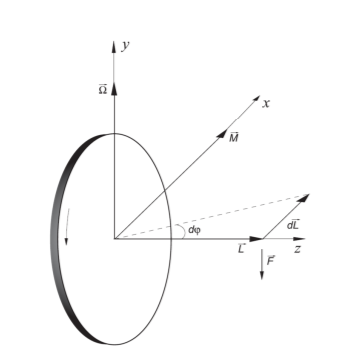
\includegraphics [scale=1]{mahovik.png}}
		\caption{Маховик}
	\end{figure}
	
	
	С этим связана замечательная устойчивость, которую приобретает движение гироскопа после приведения его в быстрое вращение. 
	Выясним, какие силы надо приложить к гироскопу, чтобы изменить 
	направление его оси. Рассмотрим для 
	примера маховик, вращающийся вокруг оси $ z $, перпендикулярной к плоскости маховика (Pис. 1). Будем считать, что
	
	\begin{equation}
		\omega_z = \omega_0, \;\;\;\;\; \omega_x = 0, \;\;\;\;\; \omega_y = 0.
	\end{equation}
	
	\noindent Пусть ось вращения повернулась в плоскости $ zx $ по направлению к оси $ x $ на бесконечно малый угол $ d\varphi $. Такой поворот означает добавочное вращение маховика вокруг оси $ y $, так что
	
	\begin{equation}
		d\varphi=\Omega dt,
	\end{equation}
	где $ \Omega $ -- угловая скорость такого вращения. Будем предполагать, что
	
	\begin{equation}
		L_\Omega \ll L_{\omega_0}
		\label{five}
	\end{equation}
	Это означает, что момент импульса маховика, равный $ I_z\omega_0 $ до приложения внешних сил, только повернётся в плоскости $ zx $ по направлению к оси $ x $, не изменяя своей величины. Таким образом, 
	
	\begin{equation}
		\left|d\vec{L}\right| = Ld\varphi = L\Omega dt.
	\end{equation}
	Но это изменение направлено вдоль оси $ x $, поэтому вектор $ d\vec{L} $ можно представить в виде векторного произведения вектора угловой скорости $ \omega $, направленного вдоль оси $ y $, на вектор собственного момента импульса маховика, направленного вдоль оси $ z $,
	
	\begin{equation}
		d\vec{L}=\vec{\Omega} \times \vec{L} dt,
	\end{equation}
	т. е.
	
	\begin{equation}
		\frac{d\vec{L}}{dt} = \vec{\Omega} \times \vec{L}.
	\end{equation}
	В силу \eqref{two} имеем
	
	\begin{equation}
		\vec{M} = \vec{\Omega} \times \vec{L}.
		\label{six}
	\end{equation}
	Формула \eqref{six} справедлива, если выполнено условие \eqref{five}. Она позволяет определить момент сил $ \vec{M} $, который необходимо приложить к маховику для того, чтобы вызвать вращение оси маховика с угловой скоростью $ \vec{\Omega} $. Мы видим, таким образом, что для поворота оси вращающегося маховика к оси $ x $ необходимо приложить силы, направленные не вдоль оси $ x $, а вдоль оси $ y $, так чтобы их момент $ \vec{M} $ был направлен вдоль оси $ x $.
	
	Для гироскопа массой $ m_\text{г} $, у которого ось собственного вращения наклонена на угол $ \alpha $ от вертикали, скорость прецессии, происходящей вокруг вертикальной оси под действием силы тяжести, равна
	
	\begin{equation}
		\Omega = \frac{M}{I_z\omega_0\sin \alpha} = \frac{m_\text{г}gl_\text{ц}\sin\alpha}{I_z\omega_0\sin\alpha} = \frac{m_\text{г}gl_\text{ц}}{I_z\omega_0},
	\end{equation}
	где $ l_\text{ц} $ -- расстояние от точки подвеса до центра масс гироскопа, т. е. скорость прецессии не зависит от угла $ \alpha $.
	
	Для изучения регулярной прецессии уравновешенного гироскопа к его оси подвешивают дополнительные грузы. Это смещает общий центр масс и создает момент сил тяжести, вызывающий прецессию. Скорость прецессии в этом случае равна
	
	\begin{equation}
		\Omega = \frac{mgl}{I_z\omega_0},
		\label{eight}
	\end{equation}
	где $ m $ -- масса груза, $ l $ -- расстояние от центра карданова подвеса до точки крепления груза на оси гироскопа.
	
	Измерение скорости прецессии гироскопа позволяет вычислить угловую скорость вращения его ротора. Расчет производится по формуле \eqref{eight}. Момент инерции ротора относительно оси симметрии $ I_0 $ измеряется по крутильным колебаниям точной копии ротора, подвешиваемой вдоль оси симметрии на жесткой проволоке. Период крутильных колебаний $ T_0 $ зависит от момента инерции $ I_0 $ и модуля кручения проволоки $ f $:
	
	\begin{equation}
		T_0 = 2\pi\sqrt{\frac{I_0}{f}}.
		\label{nine}
	\end{equation} 
	
	Чтобы исключить модуль кручения проволоки, вместо ротора гироскопа к той же проволоке подвешивают цилиндр правильной формы с известными размерами и массой, для которого легко можно вычислить момент инерции $ I_\text{ц} $. Для определения момента инерции ротора гироскопа имеем 
	
	\begin{equation}
		I_0=I_\text{ц}\frac{T_0^2}{T_\text{ц}^2},
		\label{ten}
	\end{equation}
	где $ T_\text{ц} $ --период крутильных колебаний цилиндра.
	
	\newpage
	
	
	\textbf{Ход работы:} \\
	\\
		Для определения частоты вращения ротора гироскопа будем исследовать зависимость скорости прецессии гироскопа от момента силы, действующей на его ось.
			\begin{enumerate}
		\item Отклоним ось гироскопа на 6$^{\circ}$ вверх от горизонтальной оси. Будем вешать грузы различной массы на ось гироскопа и измерять время, за которое ось гироскопа опуститься на 6$^{\circ}$ ниже горизонтальной оси. Результаты измерений занесем в таблицы \\1 - 7. ($\sigma_t=0,4$ c $\sigma_m=0.1$ г)\\
		\begin{minipage}{0.4\textwidth}
			\begin{longtable}{|c|c|c|}
				
				\hline 
				№ & $N$, обор. & $t$, с \\
				\hline
				1 & 14 & 410,0\\
				\hline
				2 & 14 & 411,0 \\
				\hline
				\caption{Масса: $m$ = 341,8 г.}
			\end{longtable}
		\end{minipage}
		\begin{minipage}{0.4\textwidth}
			\begin{longtable}{|c|c|c|}
				\hline 
				№ & $N$, обор. & $t$, с \\
				\hline
				1 & 13 & 488,1\\
				\hline
				2 & 13 & 487,3 \\
				\hline
				\caption{Масса: $m$ = 272,0 г.}
			\end{longtable}
		\end{minipage}
		\\
		\begin{minipage}{0.4\textwidth}
			\begin{longtable}{|c|c|c|}
				
				\hline 
				№ & $N$, обор. & $ t$, с \\
				\hline
				1 & 11 & 511,4\\
				\hline
				2 & 11 & 507,8 \\
				\hline
				\caption{Масса: $m$ = 219,5 г.}
				
			\end{longtable}
		\end{minipage}
		\begin{minipage}{0.4\textwidth}
			\begin{longtable}{|c|c|c|}
				\hline 
				№ & $N$, обор. & $t$, с \\
				\hline
				1 & 9 & 534,7\\
				\hline
				2 &9 & 534,1\\
				\hline
				\caption{Масса: $m$ = 175.7 г.}
			\end{longtable}
		\end{minipage}
	
		\begin{minipage}{0.4\textwidth}
		\begin{longtable}{|c|c|c|}
			\hline 
			№ & $N$, обор. & $t$, с \\
			\hline
			1 & 7 & 508,1\\
			\hline
			2 &7 & 506,3\\
			\hline
			\caption{Масса: $m$ = 141,0 г.}
		\end{longtable}
	\end{minipage}
		\begin{minipage}{0.4\textwidth}
		\begin{longtable}{|c|c|c|}
			\hline 
			№ & $N$, обор. & $t$, с \\
			\hline
			1 & 5 & 444,3\\
			\hline
			2 & 5 & 443,3 \\
			\hline
			\caption{Масса: $m$ = 115,8 г.}
		\end{longtable}
	\end{minipage}
	
	\begin{longtable}{|c|c|c|}
		\hline 
		№ & $N$, обор. & $t$, с \\
		\hline
		1 & 4 & 444,6\\
		\hline
		2 & 4 & 444,8 \\
		\hline
		\caption{Масса: $m$ = 92,7 г.}
	\end{longtable}

	 \item Посчитаем значения момента силы по следующей формуле: $M = mgl.$ \\
	  Тогда:
		$\sigma_M = M \frac{\sigma_\text{m}}{m}$, так как $l$ известно и имеет значение $l$=122мм.
	\item Скорость прецессии гироскопа найдем по формуле:	$\Omega = \frac{2\pi}{T}.$ \\Тогда: $\sigma_{\Omega}=\Omega\frac{\sigma_T}{T} $
	
	Полученные результаты записываем в таблицу 8.
	\newpage
	\begin{longtable}{|c|c|c|c|c|c|c|}
		\hline 		
		m,г &$\text{M, мН м} $ & $\overline T$, с&$\Omega$, $\text{рад} \text{ c}^{-1}\cdot10^{-3}$ &$\sigma_\text{T}$,c &$\sigma_\text{M}$, $\text{мН м} $& $\sigma_{\Omega}$, $\text{рад} \text{ c}^{-1}\cdot10^{-3}$ \\
		\hline
		92,7&113,1&110,50&56,88&0,02&0,1&0,01\\
		\hline
		115,8 &141,2 & 88,40 &71,01 & 0,02&0,1&0,01\\
		\hline
		141,0 & 172,0& 72,57 &86,57&0,03&0,1&0,03\\
		\hline
		175,7 & 214,3& 58,11 &108,14&0,03&0,1&0,05\\
		\hline
		219,5 & 267,8& 46,45 &135,2&0,04&0,1&0,1\\
		\hline
		272,0 & 331,8& 37,53 &167,4&0,06&0,1&0,1\\
		\hline
		341,8 & 416,9& 29,28 &209,4&0,07&0,1&0,2\\
		\hline
		\caption{Полученные данные}
	\end{longtable}
	
	\item По полученным данным построим график зависимости $\Omega$ от $M$ по МНК.(Рис.2)
	\item Коэффициент $ k $ наклона прямой и его погрешность вычислим  по МНК.
	Таким образом, получаем:
	
	$k =\left( 0,505 \pm 0,004 \right) \frac{\text{рад}}{\text{Дж} \cdot \text{с}}$\\
	
	
	\begin{figure}[H]
	\center{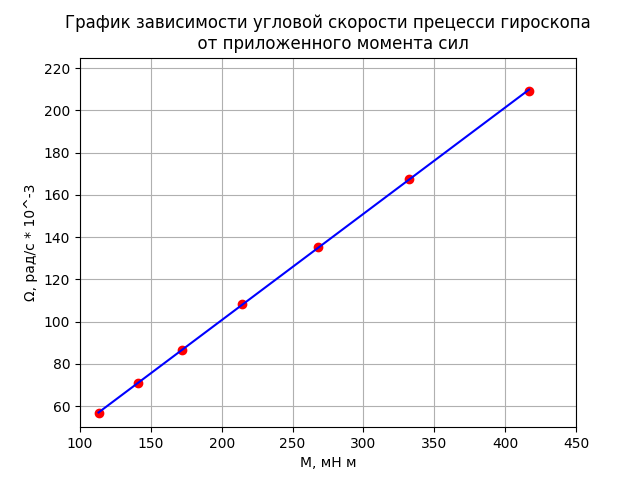
\includegraphics [scale=0.7]{first4.png}}
	\caption{}
	\end{figure}
	
	\item Вычислим момент инерции цилиндра по формуле:\\
	\\
	$I_\text{ц} = \frac{1}{2}m_\text{ц}\left( \frac{d}{2}\right)^2,$\\
		$	\sigma_{I_\text{ц}} = I_\text{ц}\sqrt{\left( \frac{\sigma_{m_{\text{ц}}}}{m_\text{ц}} \right)^2 + \left(2 \frac{\sigma_d}{d} \right)^2 } $
		
	где $ m_\text{ц} $ -- масса цилиндра, $ d $ -- его диаметр.
	\item Измерим массу и диаметр цилиндра.
		 $ m_\text{ц} = \left( 1617,8 \pm 0,1\right) $ г, 
	$ d = \left( 78,4 \pm 0,1 \right) $ мм

	В итоге получаем: $ I_\text{ц} = \left(1230 \pm 3 \right)\cdot 10^{-6} \text{ кг} \cdot \text{м}^2 $
	\item Измерим период крутильных колебаний цилиндра и ротора гироскопа, чтобы вычислить момент инерции ротора гироскопа по  формуле $I_0=I_\text{ц}\frac{T_0^2}{T_\text{ц}^2}$\\
	$	\sigma_{I_0} = I_0\sqrt{\left( \frac{\sigma_{I_{\text{ц}}}}{I_\text{ц}} \right)^2 + \left(2 \frac{\sigma_{T_0}}{T_0} \right)^2+ \left(2 \frac{\sigma_{T_{\text{ц}}}}{T_{\text{ц}}} \right)^2 } $
	
	
	\begin{minipage}{0.4\textwidth}
		\begin{longtable}{|c|c|c|c|}
			\hline 
			№ & $N$, колебаний & $t$, с& $T$, c\\
			\hline
			1 & 10 & 40,4&4,04\\
			\hline
			2 &10 & 40,2&4,02\\
			\hline
			3 &10 & 40,2&4,02\\
			\hline
			\caption{Данные цилиндра}
		\end{longtable}
	\end{minipage}
	\begin{minipage}{0.4\textwidth}
		\begin{longtable}{|c|c|c|c|}
			\hline 
			№ & $N$, колебаний & $t$, с& $T$, c\\
			\hline
			1 & 10 & 31,7&3,17\\
			\hline
			2 &10 & 31,7&3,17\\
			\hline
			3 &10 & 31,8&3,18\\
			\hline
			\caption{Данные ротора}
		\end{longtable}
	\end{minipage}
	\\ где: $\sigma_t=0,4$c,  $\sigma_T=0,04$c\\
       В итоге получаем: 
	
		$I_0=(78\pm2)\cdot 10^{-5}\text{ кг} \cdot \text{м}^2.$
	

	\item Рассчитаем частоту вращения ротора гироскопа по формуле:	$\nu = \frac{\omega_0}{2\pi}$, где
	
	 $\omega_0 = \frac{mgl}{I_0\Omega} = \frac{1}{I_0 k}$, \\ 
	
	$\sigma_{\omega_0} = \omega_0\sqrt{\left( \frac{\sigma_{I_{\text{0}}}}{I_\text{0}} \right)^2 + \left( \frac{\sigma_{\Omega}}{\Omega} \right)^2+ \left( \frac{\sigma_{m}}{m} \right)^2 } $
	
	$	\sigma_\nu = \nu \frac{\sigma_{\omega_0}}{\omega_0}$
	
	$\omega_0 =\left( 2521 \pm 65 \right) \text{рад с}^{-1}$\\
	
	Получим частоту:  $\nu = \left( 399 \pm 10 \right) \text{ Гц}$
	
	
	
	\item Определим момент силы трения, из-за которого опускается рычаг гироскопа с грузом.
	
	$\Omega_{\text{тр}} = 2\alpha/t$ -- угловая скорость прецессии гироскопа под действием момента силы трения, где $\alpha$ -- начальный угол отклонения оси гироскопа (равен конечному), $t$ -- время, за которое рычаг гироскопа опустился на угол $2\alpha$.
	
	$M_{F_{\text{тр}}} =\Omega_{\text{тр}} I_{0}\omega_{0}$
	
	$M_{F_{\text{тр}}} = \frac{ I_{0}\omega_{0}\pi \arcsin\left(\frac{\Delta h}{l}\right)}{90^{\circ} t}$, где $\Delta h$=12,8 мм -- расстояние, на которое поднят рычаг гироскопа относительно горизонтального положения.
	
	 $\sigma_{M_{ F_{\text{тр}}}} = \sqrt{(\frac{\partial f}{\partial I_0}\sigma_{I_0})^2 + (\frac{\partial f}{\partial \omega_0}\sigma_{\omega_0})^2+(\frac{\partial f}{\partial \Delta h}\sigma_{\Delta h})^2 +(\frac{\partial f}{\partial t}\sigma_t)^2}$
	
	Получим $M_{F_{\text{тр}}}= (8,8\pm 0,2)\cdot 10^{-4}$ Н м
	
	
	\item Определим частоту вращения ротора гироскопа по фигурам Лиссажу с помощью осциллографа. Изменяя частоту генератора и отключая питание от гироскопа, на экране осциллографа получим неподвижный эллипс, так же посчитаем время за которое эллипс стал устойчивым. Данные занесем  в таблицу 11, построим график по полученным значениям (Рис3.). По МНК получим коэффициент b  и эго погрешность, так мы определим значение $\nu$ при t=0. \\ \\
	
	\begin{longtable}{|c|c|c|c|c|c|c|c|c|c|}
		\hline 
		№ & 1 & 2 & 3& 4&5&6&7&8&9\\
		\hline
		$\nu$, Гц & 390 & 380 &370&360&350&340&330&320&310\\
		\hline
		t, c &9,5 &43,7 &83,0& 107,3&150,3&181,5&210,7&251,7&293,4\\
		\hline
		\caption{Значения $\nu$ и t}
		$\sigma_t=0,4$c
	\end{longtable}
		\end{enumerate}
	Получаем: $\nu=392\pm2$ Гц
	
	\begin{figure}[H]
		\center{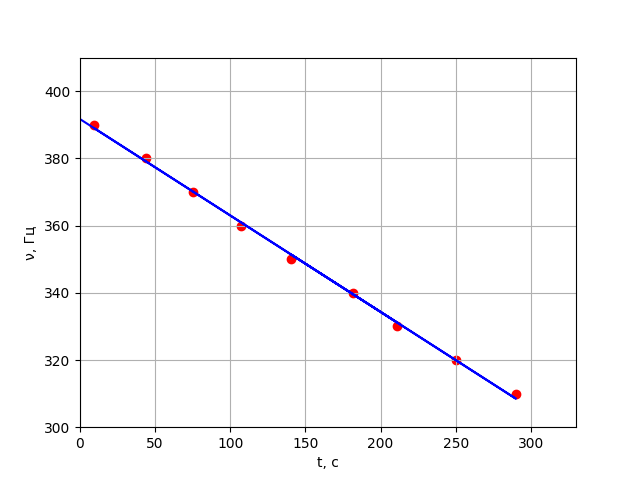
\includegraphics [scale=0.7]{first5.png}}
		\caption{График частоты от времени}
		\end{figure}
	
	
		\textbf{Вывод:}
	В данной работе мы исследовали вынужденную прецессию гироскопа, установили зависимость скорости вынужденной прецессии от величины момента сил, действующих на ось гироскопа, определили частоту вращения ротора гироскопа 2 способами и получили одинаковые значения в пределах погрешности.
	

	
\end{document}